\section{Introduction}
Recent advancements in large language model (LLM) agents have focused primarily on improving their capabilities in complex task execution—ranging from code debugging and repository management to autonomous web browsing. While these functionalities are crucial, another foundational yet underexplored dimension is memory: the ability of agents to persist, retrieve, and utilize past user-specific information over time. Human cognition relies heavily on memory—recalling conversations, recognizing patterns, and adapting behavior based on prior experience. Analogously, memory mechanisms in LLM agents are essential for delivering consistent, personalized interactions, learning from feedback, and avoiding repetitive queries.
However, most LLM-based personal assistants remain stateless beyond their current prompt window, retaining no lasting memory unless context is explicitly re-provided. This limitation hinders their long-term usability, especially in real-world settings where users expect assistants to evolve, recall, and personalize over time \cite{lscs}.

To address this, a range of memory-augmented systems have been proposed. One common approach is the use of knowledge graphs, as seen in systems like Zep~\citep{zep} and Cognee~\citep{cognee}. These frameworks are well-suited for representing structured relationships between entities but struggle to model sequential events, emotional states, full-length documents, or multi-modal inputs such as images. Another approach involves flattened memory architectures that store and retrieve textual chunks using vector databases. Examples include Letta~\citep{memgpt}, Mem0~\citep{mem0}, and ChatGPT’s memory system. Letta divides its memory into components—recall memory for conversation history, core memory for preferences, and archival memory for long documents—while ChatGPT focuses primarily on core and recall memories. Mem0 adopts a memory system that contains flattened facts distilled from the user inputs, which serves similar roles as Letta's archival memory while being more distilled. While prevalent, these memory systems face several challenges: (1) Lack of compositional memory structure: Most approaches store all historical data in a single flat store without routing into specialized memory types (e.g., procedural, episodic, semantic), making retrieval inefficient and less accurate. (2) Poor multi-modal support: Text-centric memory mechanisms fail when the majority of the input is non-verbal (e.g., images, interface layouts, maps). (3) Scalability and abstraction: Storing raw inputs, especially images, leads to prohibitive memory requirements, with no effective abstraction layer to summarize and retain only salient information. 

\begin{figure*}
    \centering
    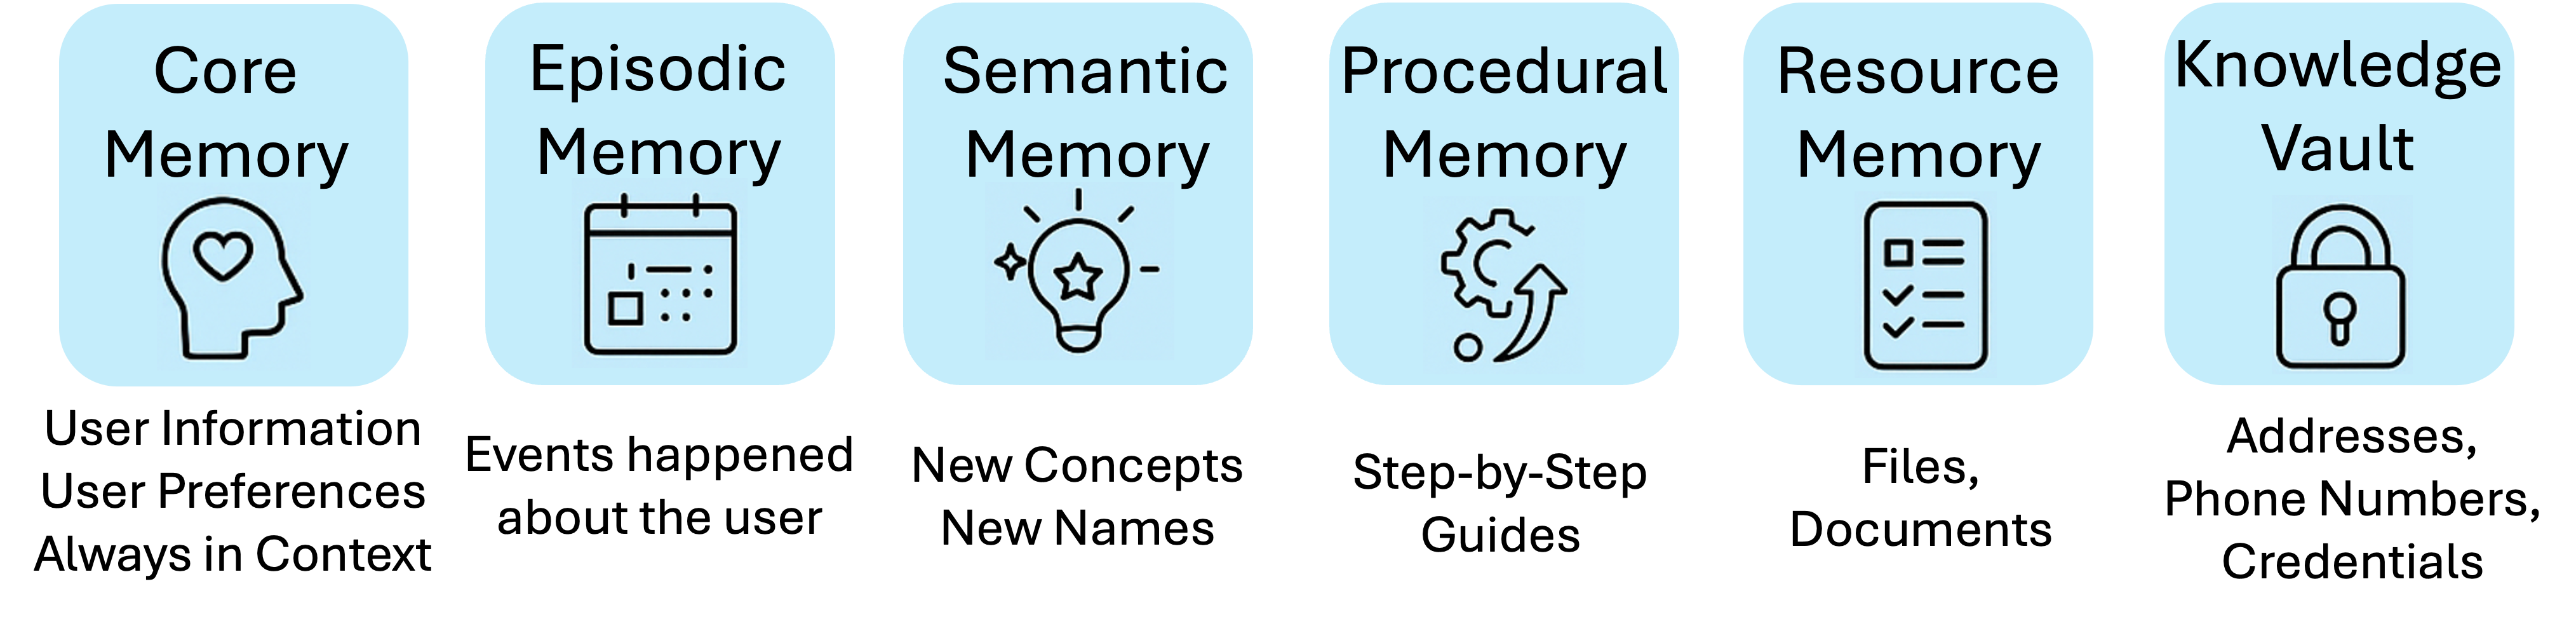
\includegraphics[width=\linewidth]{figures/six_memory_components.png}
    \caption{The six memory components of \ours, each providing specialized functionality.}
    \label{fig:overall_structure}
\end{figure*}


To address the limitations of existing memory systems, we argue that effective \textbf{Routing} and \textbf{Retrieving} are the key capabilities a memory-augmented agent must possess. Most current systems focus primarily on Short-Term and Long-Term Memory~\citep{memgpt,caim,cognitive_memory_in_llms}, with some incorporating Mid-Term Memory~\citep{memoryos}. In contrast, we draw inspiration from works that explore more specialized memory types, including episodic memory~\citep{episodic_memory_missing_piece,echo,arigraph}, semantic memory~\citep{memory_consciousness_and_llm}, and procedural memory~\citep{procedural_memory_all_you_need}. Building on these foundations, we propose a more comprehensive architecture consisting of six memory components: \textbf{Core Memory}, \textbf{Episodic Memory}, \textbf{Semantic Memory}, \textbf{Procedural Memory}, \textbf{Resource Memory}, and the \textbf{Knowledge Vault} (As shown in Figure \ref{fig:overall_structure}).
% Episodic, Semantic, and Procedural Memory follow prior formulations. 
Episodic Memory stores user-specific events and experiences; Semantic Memory captures concepts and named entities (e.g., the meaning of a new phrase or an understanding of a person); Procedural Memory records step-by-step instructions for performing tasks. Resource Memory is designed to store documents, files, and other media shared by the user. Knowledge Vault holds critical verbatim information that must be preserved exactly, such as addresses, phone numbers, email accounts, and other sensitive facts.

Each memory component is internally organized using a hierarchical structure. For example, Episodic Memory includes fields such as \texttt{summary} and \texttt{details}, while Semantic Memory organizes information by \texttt{name} and \texttt{description}. Managing this structured and heterogeneous memory is challenging for a single agent. Therefore, we adopt a multi-agent architecture: six Memory Managers for six memory components, and a \textbf{Meta Memory Manager} responsible for task routing. While this memory system can be plugged and connected with other existing agents, we build an extra \textbf{Chat Agent} to demonstrate how we can interact with an agent that has access to our memories. This memory system, which we call \textbf{\ours}, is modular and designed as a comprehensive and full memory system for LLM-based agents. Moreover,
when interacting with the Chat Agent, we propose an Active Retrieval mechanism, where the agent is required to generate a \emph{topic} before answering the question or executing the next step, and the retrieved information is inputted into the model in the system prompt. Meanwhile, we design multiple retrieval tools so that the agent can choose appropriate ones in response to different situations.

We evaluate \ours in two experimental settings. First, we introduce a challenging benchmark that requires extracting information and building memory from multimodal input. To this end, we collect between 5,000 and 20,000 high-resolution screenshots spanning one month of computer usage from three PhD students and construct evaluation questions grounded in their visual activity history. This setting demands sophisticated memory modeling and exceeds the capacity of existing long-context models. For example, each screenshot ranges from 2K to 4K resolution depending on the user's monitor, which limits Gemini to processing no more than 500 images at full resolution or approximately 3,600 images when resized to 256×256 pixels. Second, following Mem0~\citep{mem0}, we assess performance on the LOCOMO dataset~\citep{locomo}, which comprises long-form, multi-turn conversations. While each conversation is relatively short (around 26,000 tokens on average), we constrain the Chat Agent to answer questions using only retrieved memories, without access to the original conversation transcripts. This setup enables us to evaluate whether our system can effectively distill and route essential information into memory. In terms of results, because no existing memory systems can handle such a large volume of multimodal input, we compare against retrieval-augmented generation (RAG) baselines and long-context baselines. \ours achieves a 35\% improvement over RAG baselines while reducing storage requirements by 99.9\%, and a 410\% improvement over long-context baselines with a 93.3\% reduction in storage. On LOCOMO, \ours reaches state-of-the-art performance with an overall accuracy of 85.38\%, outperforming the best existing method by 8.0\% and approaching the upper bound set by long-context models. 
To make our memory system more accessible, we also developed a personal assistant powered by \ours. With the user’s permission to capture screen content, the assistant continuously builds a memory from screenshots and can answer any questions related to this accumulated information. This represents our effort to bring advanced memory capabilities to everyone, enabling users to experience the benefits of our system firsthand.

Our contributions are summarized as follows:
\begin{itemize}[leftmargin=*]
\item We analyze the limitations of existing memory architectures for LLM-based agents and propose a novel memory system composed of six specialized components and eight different agents. 
\item We introduce a new benchmark in which the agent must interpret a large collection of screenshots to build an understanding of user behavior—posing a significant challenge to the memory.
\item Through experiments on our new benchmark and existing benchmark LOCOMO, we demonstrate that \ours significantly outperform existing memory systems.
\item To make our approach accessible, we build and release a personal assistant application powered by \ours, enabling users to experience advanced memory capabilities in real-world scenarios.
\end{itemize}




